\ifx\boi\undefined\ifx\problemname\undefined
\providecommand\sampleinputname{}
\providecommand\sampleoutputname{}
\documentclass[german]{templates/boi}
\problemlanguage{.de}
\fi
\newcommand{\boi}{Baltische Informatikolympiade}
\newcommand{\practicesession}{Practice Session}
\newcommand{\contestdates}{27. April - 1. Mai, 2018}
\newcommand{\dayone}{Tag 1}
\newcommand{\daytwo}{Tag 2}
\newcommand{\licensingtext}{Diese Aufgabenstellung ist unter der CC BY-SA 4.0 lizensiert.}
\newcommand{\problem}{Aufgabe}
\newcommand{\inputsection}{Eingabe}
\newcommand{\outputsection}{Ausgabe}
\newcommand{\interactivity}{Interaktivität}
\newcommand{\grading}{Grading}
\newcommand{\scoring}{Scoring}
\newcommand{\constraints}{Beschränkungen}
\renewcommand{\sampleinputname}{Beispieleingabe}
\renewcommand{\sampleoutputname}{Beispielausgabe}
\newcommand{\sampleexplanation}[1]{Beschreibung zu Beispiel #1}
\newcommand{\sampleexplanations}{Beschreibung der Beispiele}
\newcommand{\timelimit}{Zeitlimit}
\newcommand{\memorylimit}{Speicherlimit}
\newcommand{\seconds}{s}
\newcommand{\megabytes}{MB}
\newcommand{\group}{Gruppe}
\newcommand{\points}{Punkte}
\newcommand{\limitsname}{Limits}
\newcommand{\additionalconstraints}{Zusätzliche Beschränkungen}
\newcommand{\testgroups}{
Deine Lösung wird auf mehreren Testgruppen ausgeführt werden, von denen jede eine bestimmte Punktzahl wert ist.
Jede Testgruppe enthält mehrere Testcases. Um Punkte für eine Testgruppe zu bekommen, müssen alle Testfälle in der entsprechenden Gruppe gelöst werden.
Deine finale Punktzahl wird die maximal erreichte Punktzahl in allen Einsendungen sein.
}
\fi
\def\version{jury-1}
\problemname{Liebespolygon}
Wie wir alle wissen, können Seifenopern mit vielen Protagonisten zu ernsthaft komplizierten Liebesdramen führen. In einer TV-Serie gibt es $N$ Protagonisten. Jeder Protagonist liebt exakt einen anderen Protagonisten (der auch er selbst sein kann). Zwei Protagonisten sind in einer Liebesbeziehung genau dann, wenn sie sich gegenseitig lieben.

Ein besonders komplizierter Beziehungstyp ist ein ``Liebespolygon''. 3 oder mehr Protagonisten sind in einem ``Liebespolygon'', wenn der erste Protagonist den zweiten liebt, der zweite Protagonist den dritten und so weiter, und der letzte Protagonist auch den ersten liebt.

Neue Umfragen haben gezeigt, dass Fernsehzuschauer von diesem Drama gelangweilt sind und etwas romantischeres bevorzugen würden.

Daher wurde entschieden, einige Charaktere mit Liebespfeilen zu beschießen, sodass jeder in einer Beziehung ist.
Wie viele Liebespfeile werden mindestens benötigt, um das zu erreichen?

\section*{\inputsection}
Die erste Zeile der Eingabe enthält eine ganze Zahl $N$, die Anzahl der involvierten Charaktere.
Die nächsten $N$ Zeilen enthalten jeweils zwei durch Leerzeichen getrennte Namen $s$ und $t$, die dafür stehen, dass der Charakter mit Namen $s$ zu Beginn den mit Namen $t$ liebt.
Die Namen der Charaktere sind nicht länger als $10$ Zeichen und bestehen nur aus englischen Kleinbuchstaben.

\section*{\outputsection}
Gebe eine ganze Zahl aus: Die minimale Anzahl von Liebespfeilen, die benötigt werden, um jede Person in eine Beziehung zu bekommen.
Falls das nicht möglich ist, gebe $-1$ aus.

\section*{\constraints}
\testgroups

\noindent
\begin{tabular}{| l | l | l | l |}
\hline
\group & \points & \limitsname & \additionalconstraints \\ \hline
1     & 21     & $2 \le N \le 20$ & \\ \hline
2     & 25     & $2 \le N \le 100\,000$ & Jede Person wird von jemandem geliebt. \\ \hline
3     & 29     & $2 \le N \le 100\,000$ & Es gibt keine Beziehungen oder ``Liebespolygone''. \\ \hline
4     & 25     & $2 \le N \le 100\,000$ & \\ \hline
\end{tabular}

\section*{\sampleexplanations}

\begin{center}
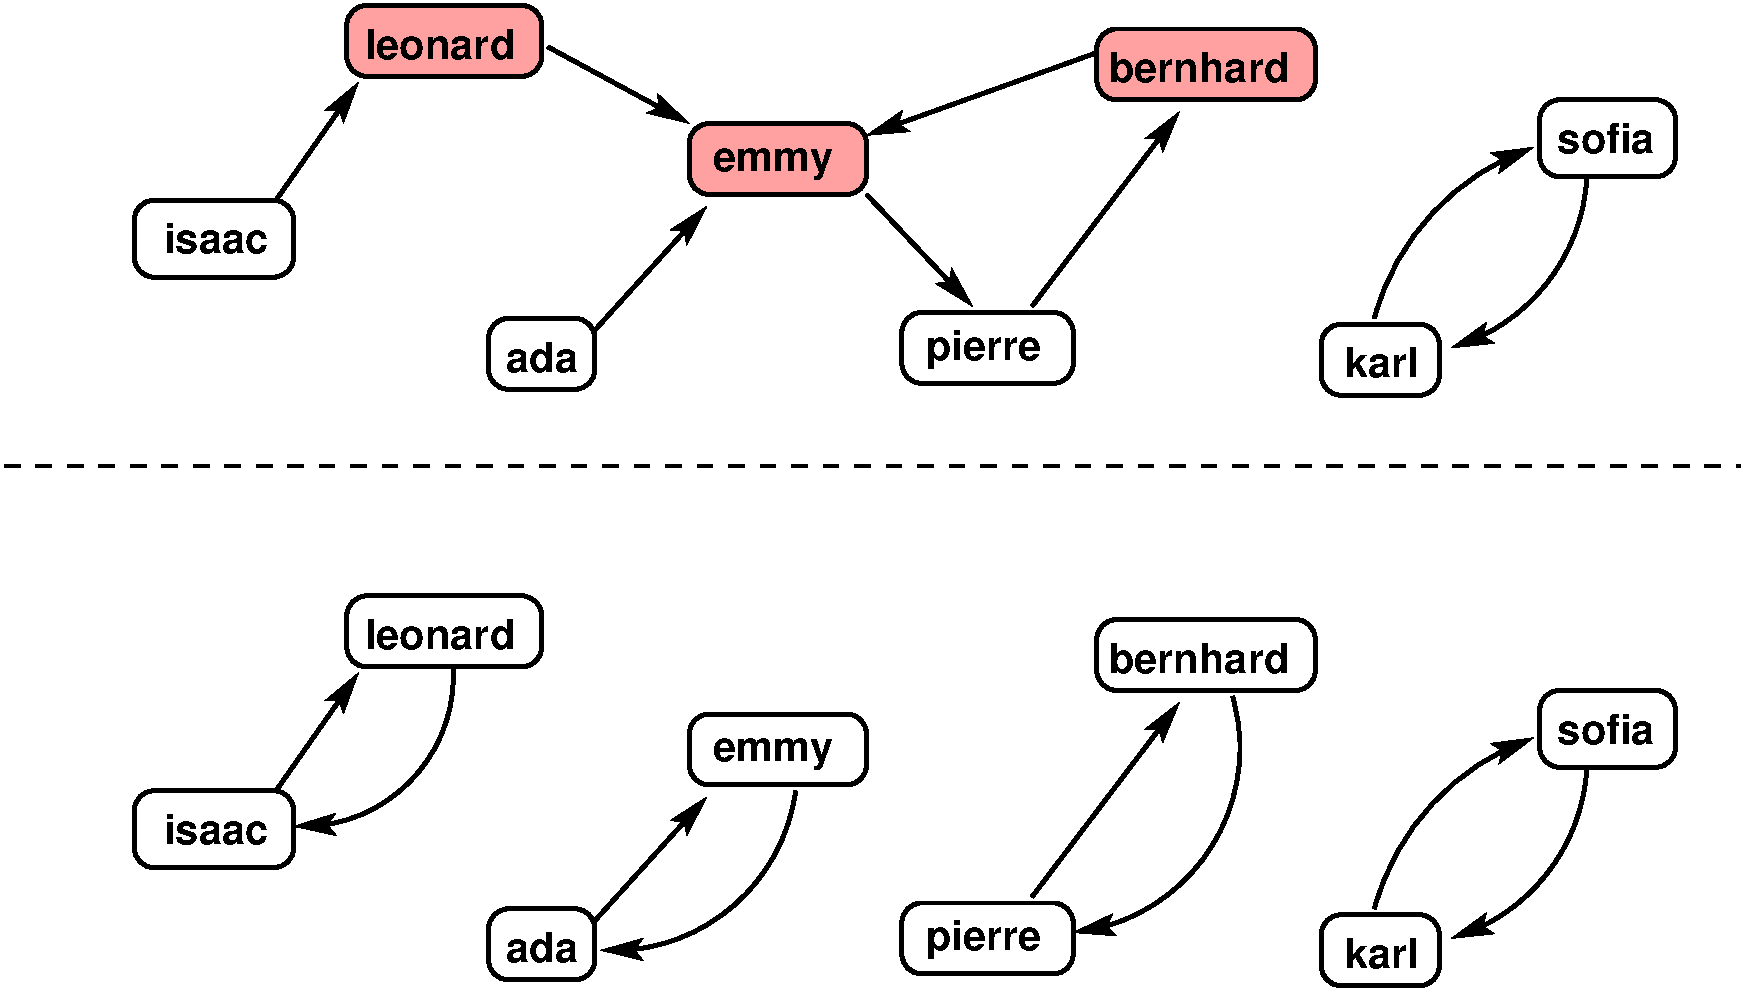
\includegraphics[width=0.5\textwidth]{polygonfig.pdf}
\end{center}

Das erste Beispiel ist in der Abbildung oben dargestellt.
Der obere Teil zeigt die Situation zu Beginn, wobei ein Pfeil von $s$ nach $t$ angibt, dass $s$ zu Beginn $t$ liebt. Die rosa Farbe gibt an, welche Charaktere in der eindeutigen optimalen Lösung mit Liebespfeilen beschossen werden müssen.
Der untere Teil zeigt die Situation nachher.

Im zweiten Beispiel (welches die Beschränkungen der Gruppe 3 erfüllt), gibt es mehrere optimale Lösungen.
Eine davon ist es, Personen \texttt{a}, \texttt{b} und \texttt{d} mit Liebespfeilen zu beschießen, und in \texttt{b}, \texttt{a} bzw. \texttt{c} zu verlieben.

Im dritten Beispiel gibt es ein Liebesdreieck. Unabhängig davon, wie viele Liebespfeile wir verschießen, wird immer jemand alleine bleiben.
